\documentclass[zihao=-4]{ctexart}

\usepackage{xeCJK}
\usepackage{amssymb}
\usepackage{amsmath}
\usepackage{graphicx}
\usepackage{booktabs}
\usepackage{array}
\usepackage{geometry}
\usepackage{fontspec}
\usepackage{setspace}
\usepackage{fancyhdr}
\usepackage{float}
\usepackage{titlesec}
\usepackage{titletoc}
\usepackage{caption}
\usepackage{changepage}
\usepackage{gbt7714}
\usepackage{enumitem}
\usepackage{hyperref}

\geometry{left=3cm,right=2cm,top=2.5cm,bottom=2.5cm,a4paper}
\graphicspath{{include_picture/}}
\bibliographystyle{gbt7714-numerical}
\hypersetup{hidelinks}

\setmainfont[
  Path=fonts/,
  BoldFont=times-new-roman-bold.ttf,
  ItalicFont=times-new-roman-italic.ttf,
  BoldItalicFont=times-new-roman-bold-italic.ttf
]{times-new-roman.ttf}
\setmonofont[Path=fonts/]{Courier New.ttf}
\setCJKfamilyfont{hwzs}[Path=fonts/]{STKzhongsong.ttf}
\newcommand{\zhongsong}{\CJKfamily{hwzs}}
\setCJKfamilyfont{hwxw}[Path=fonts/]{STKxinwei.ttf}
\newcommand{\xinwei}{\CJKfamily{hwxw}}
\newcommand{\erhao}{\fontsize{22pt}{22pt}\selectfont}
\newcommand{\sanhao}{\fontsize{16pt}{20pt}\selectfont}
\newcommand{\sihao}{\fontsize{14pt}{18pt}\selectfont}
\newcommand{\xiaosi}{\fontsize{12pt}{16pt}\selectfont}
\newcommand{\xiaowu}{\fontsize{9pt}{13pt}\selectfont}
\newcommand{\Fengru}{第三十六届“冯如杯”创意赛道}

\pagestyle{fancy}
\fancyhf{}
\setlength{\headwidth}{\textwidth}
\setlength{\headheight}{16pt}
\chead{\xiaowu 北京航空航天大学第三十六届“冯如杯”竞赛创意赛道参赛作品}
\cfoot{\thepage}

\titleformat{\section}[block]{\sanhao\heiti\centering}{\chinese{section}、}{0pt}{}
\titleformat{\subsection}[block]{\sihao\heiti}{（\chinese{subsection}）}{0pt}{}
\titlespacing{\section}{0pt}{18pt}{10pt}
\titlespacing{\subsection}{0pt}{8pt}{6pt}

\titlecontents{section}[1.8em]{\addvspace{2pt}\filright}
{\contentspush{\thecontentslabel\hspace{0.8em}}}
{}{\titlerule*[8pt]{.}\contentspage}

\titlecontents{subsection}[3.6em]{\addvspace{2pt}\filright}
{\contentspush{\thecontentslabel\hspace{0.8em}}}
{}{\titlerule*[8pt]{.}\contentspage}

\captionsetup[figure]{font={small}, labelfont=bf}

\begin{document}
\linespread{1.8}\selectfont
\setlength{\parskip}{0pt}
\setlength{\parindent}{2em}

\pagenumbering{gobble}
\renewcommand{\headrulewidth}{0pt}
\thispagestyle{empty}
\leftline{
\includegraphics[scale=1]{xiaohui.png}}
\vspace{32pt}

\begin{center}

\includegraphics[height=2.25cm,width=12.78cm]{xiaoming.png}
\end{center}

\vspace{16pt}
\begin{center}
{\fontsize{22pt}{22pt}\selectfont\zhongsong {\Fengru 项目论文}}\\[14pt]
{\erhao\zhongsong 梦拓龙虾}\\[14pt]
\end{center}
\rightline{\xinwei\sanhao ——面向校内课程持续推进的助学智能体设计与实现}

\clearpage
\pagenumbering{roman}
\section*{摘要}
\begin{spacing}{1.5}
高校课程学习真正困难的部分，往往不是某一次提问得不到回答，而是学习缺少持续推进机制。许多学生在课上获得了信息，在课后却难以及时整理重点、完成巩固、坚持复习并根据实际进展调整下一步行动。现有学习平台更擅长提供课程资源，通用聊天式人工智能更擅长即时问答，但二者都难以围绕一门具体课程长期监督学习节奏并主动推进学习过程。针对这一问题，本文设计并实现助学智能体“梦拓龙虾”。该系统依托校内课程资源平台中的课表、作业、通知、回放和课件等信息，以课程为组织单元，以课程项目与定时任务为主要抓手，将目标建立、任务推进、课后复盘、周期复习和动态调整组织为持续运行的学习支持过程。尤其在课后监督场景中，系统支持按照预设的 cron 规则，在每节课结束后的当日晚间结合最近一次课程回放内容，向学生推送核心知识点、小题或提醒信息，用于复习与阶段性评估。本文围绕课程目标建立、课后监督推送、周期复习和任务调整等典型场景对原型进行验证。结果表明，梦拓龙虾能够较好地将课程学习从零散问答转化为持续推进的过程性支持，在维持学习节奏、加强课后巩固和提升课程资源利用针对性方面具有较好的应用潜力。
\end{spacing}

\textbf{关键词：}助学智能体；课程学习推进；课后监督；复习支持；校内课程资源

\newpage
\section*{\textbf{Abstract}}
\begin{spacing}{1.5}
\begin{adjustwidth}{0.42cm}{0.42cm}
\qquad The main difficulty of university course learning often lies not in answering a single question, but in sustaining learning progress over time. Students may attend lectures and accumulate materials, yet still struggle to consolidate what they learned after class, maintain review routines, and adjust their next actions as progress changes. Existing learning platforms are good at presenting course resources, while general conversational AI is good at instant question answering; neither is naturally designed to supervise learning rhythm and continuously advance the study process of a specific course. To address this gap, this paper presents ``Mentor Lobster'', a learning-support agent for sustained course progression. Grounded in campus course platforms such as schedules, assignments, notices, lecture replays, and slides, the system uses course projects and scheduled tasks as its main organizing units, and links goal setting, task advancement, post-class reflection, periodic review, and dynamic adjustment into a continuing support process. A representative scenario is a cron-based post-class routine: on the evening after each lecture, the agent uses the most recent replay-related content to push key knowledge points, short questions, or reminders for consolidation and lightweight assessment. The prototype is validated through typical scenarios including course goal creation, post-class supervision, periodic review, and dynamic adjustment. Results show that the proposed agent can effectively turn fragmented question answering into sustained process-oriented learning support, with promising value in maintaining learning rhythm, strengthening post-class consolidation, and improving the relevance of course-resource use.

\textbf{Keywords:} educational agent, course learning progression, post-class supervision, review support, campus course resources
\end{adjustwidth}
\end{spacing}

\clearpage
\tableofcontents
\clearpage

\renewcommand{\headrulewidth}{0.4pt}
\pagenumbering{arabic}
\setcounter{page}{1}

\section{引言}
高校课程学习并不缺少信息。课表、作业、通知、课件和回放已经越来越多地沉淀在校内平台中，学生也可以随时使用通用聊天式人工智能完成概念解释、答案整理和内容总结。然而，学习效果仍然经常在课后迅速衰减，其根本原因并不在于“资料不够多”，而在于缺少一套能够持续推进学习的外部支持机制。很多学生真正遇到的困难是：上完课以后没有及时复盘，第二天开始忘记，之后再也没有被提醒回看，等到作业或考试临近才重新补救。由此可见，高校课程学习的核心矛盾并不是单次答疑能力不足，而是学习过程缺少持续监督、承接与推进。

\subsection{研究背景与问题提出}
从第一性原理看，课程学习至少包含三个连续动作：首先要知道当前这门课最值得推进的目标是什么；其次要知道此刻最应该做的下一步动作是什么；最后要在课后与后续阶段不断通过复盘和复习来保持知识。传统课堂只稳定覆盖了“上课输入”这一环节，而课后巩固、后续复习和动态调整则高度依赖学生自我管理能力。对于节奏紧张、并行课程多的高校学生而言，这恰恰是最容易失守的部分。

教育研究早已表明，持续诊断与反馈是高质量学习支持的重要来源\cite{bloom1984}；同时，分散练习与提取练习有助于提高知识保持效果\cite{cepeda2006,dunlosky2013,karpicke2011}。这意味着，如果助学系统只能回答“现在这个问题”，却不能在课后再次把学生拉回学习任务、再次触发复习和检查，就很难真正改善课程学习过程。基于这一判断，本文关注的核心问题是：能否构建一个依托校内课程资源平台、能够在课后持续监督并推进课程学习的助学智能体。

\subsection{现有方法分析}
现有方法大体可以分为三类。第一类是校内学习平台。这类平台在课程资源沉淀、课表展示和作业通知方面具备稳定优势，但它们的基本逻辑仍然是“提供信息入口”，而不是“围绕学生当前状态主动推进学习”。第二类是通用聊天式人工智能。它们能够快速解释概念、生成总结、回答问题，但默认工作方式通常是被动响应用户输入，难以长期围绕同一门课保持状态并主动监督学习节奏。第三类是通用待办和提醒工具。这类工具具备基本定时能力，却往往缺少与课程内容的绑定，难以根据具体课程回放、课件或课堂重点给出真正有针对性的课后支持。

因此，一个面向高校课程学习的有效系统，不应仅仅停留在资源整合、单轮问答或机械提醒层面，而应把课程资源、学习状态和主动推进机制结合起来。特别是在课后场景中，系统若能自动利用课程回放和课件内容生成当晚巩固任务，就比单纯的“记得复习”更接近真实有效的学习支持。

\subsection{本文思路与主要内容}
基于上述认识，本文提出助学智能体“梦拓龙虾”。其核心创意不是把系统写成一个无所不能的学习助手，而是依托校内课程资源平台，把一门课从一次次零散提问转化为持续推进的学习过程。换言之，梦拓龙虾关注的不是“回答得像不像老师”，而是“能不能在一门课上不断把学生往前推一步”。

本文的主要工作包括：一是围绕课程持续推进这一目标，给出梦拓龙虾的系统定位、总体架构与核心对象设计；二是重点设计课后监督、周期复习、动态调整以及个性化 cron 任务等关键机制；三是基于原型系统，对课程目标建立、课后监督推送、周期复习和自定义任务执行等典型场景进行验证，并分析其价值与局限。

\section{梦拓龙虾总体设计}
\subsection{智能体定位}
梦拓龙虾面向高校课程学习场景，以课内学习支持为中心，同时兼顾少量与课程密切相关的复习、检查和提醒任务。它不是通用生活管理助手，也不是单纯的课程搜索工具，而是一个围绕具体课程长期运行的过程型助学智能体。其价值并不体现在某一次回答是否完整，而体现在能否在课后、复习和阶段变化时继续发挥作用。

这一定位决定了系统必须同时满足两个条件：一方面，它要能够接入真实课程资源，而不是脱离课程上下文空谈学习方法；另一方面，它要能够在用户没有主动提问时，通过定时任务和状态更新机制继续承担监督与推进功能。只有同时满足这两点，系统才可能真正参与课程学习过程，而不是停留在答疑工具层面。

\subsection{核心创意}
梦拓龙虾的核心创意可以概括为：依托校内课程资源平台，为一门课建立可持续推进的学习支持链条。这里所谓“推进”，不是简单地连续发送提醒，而是让学习过程中的几个关键环节形成稳定承接关系，包括目标建立、任务推进、课后复盘、周期复习和动态调整。与其说这是一个已经完全自动闭合的系统，不如说它是一套能够不断把学生拉回正确学习节奏的主动支持机制。

\begin{figure}[H]
\centering
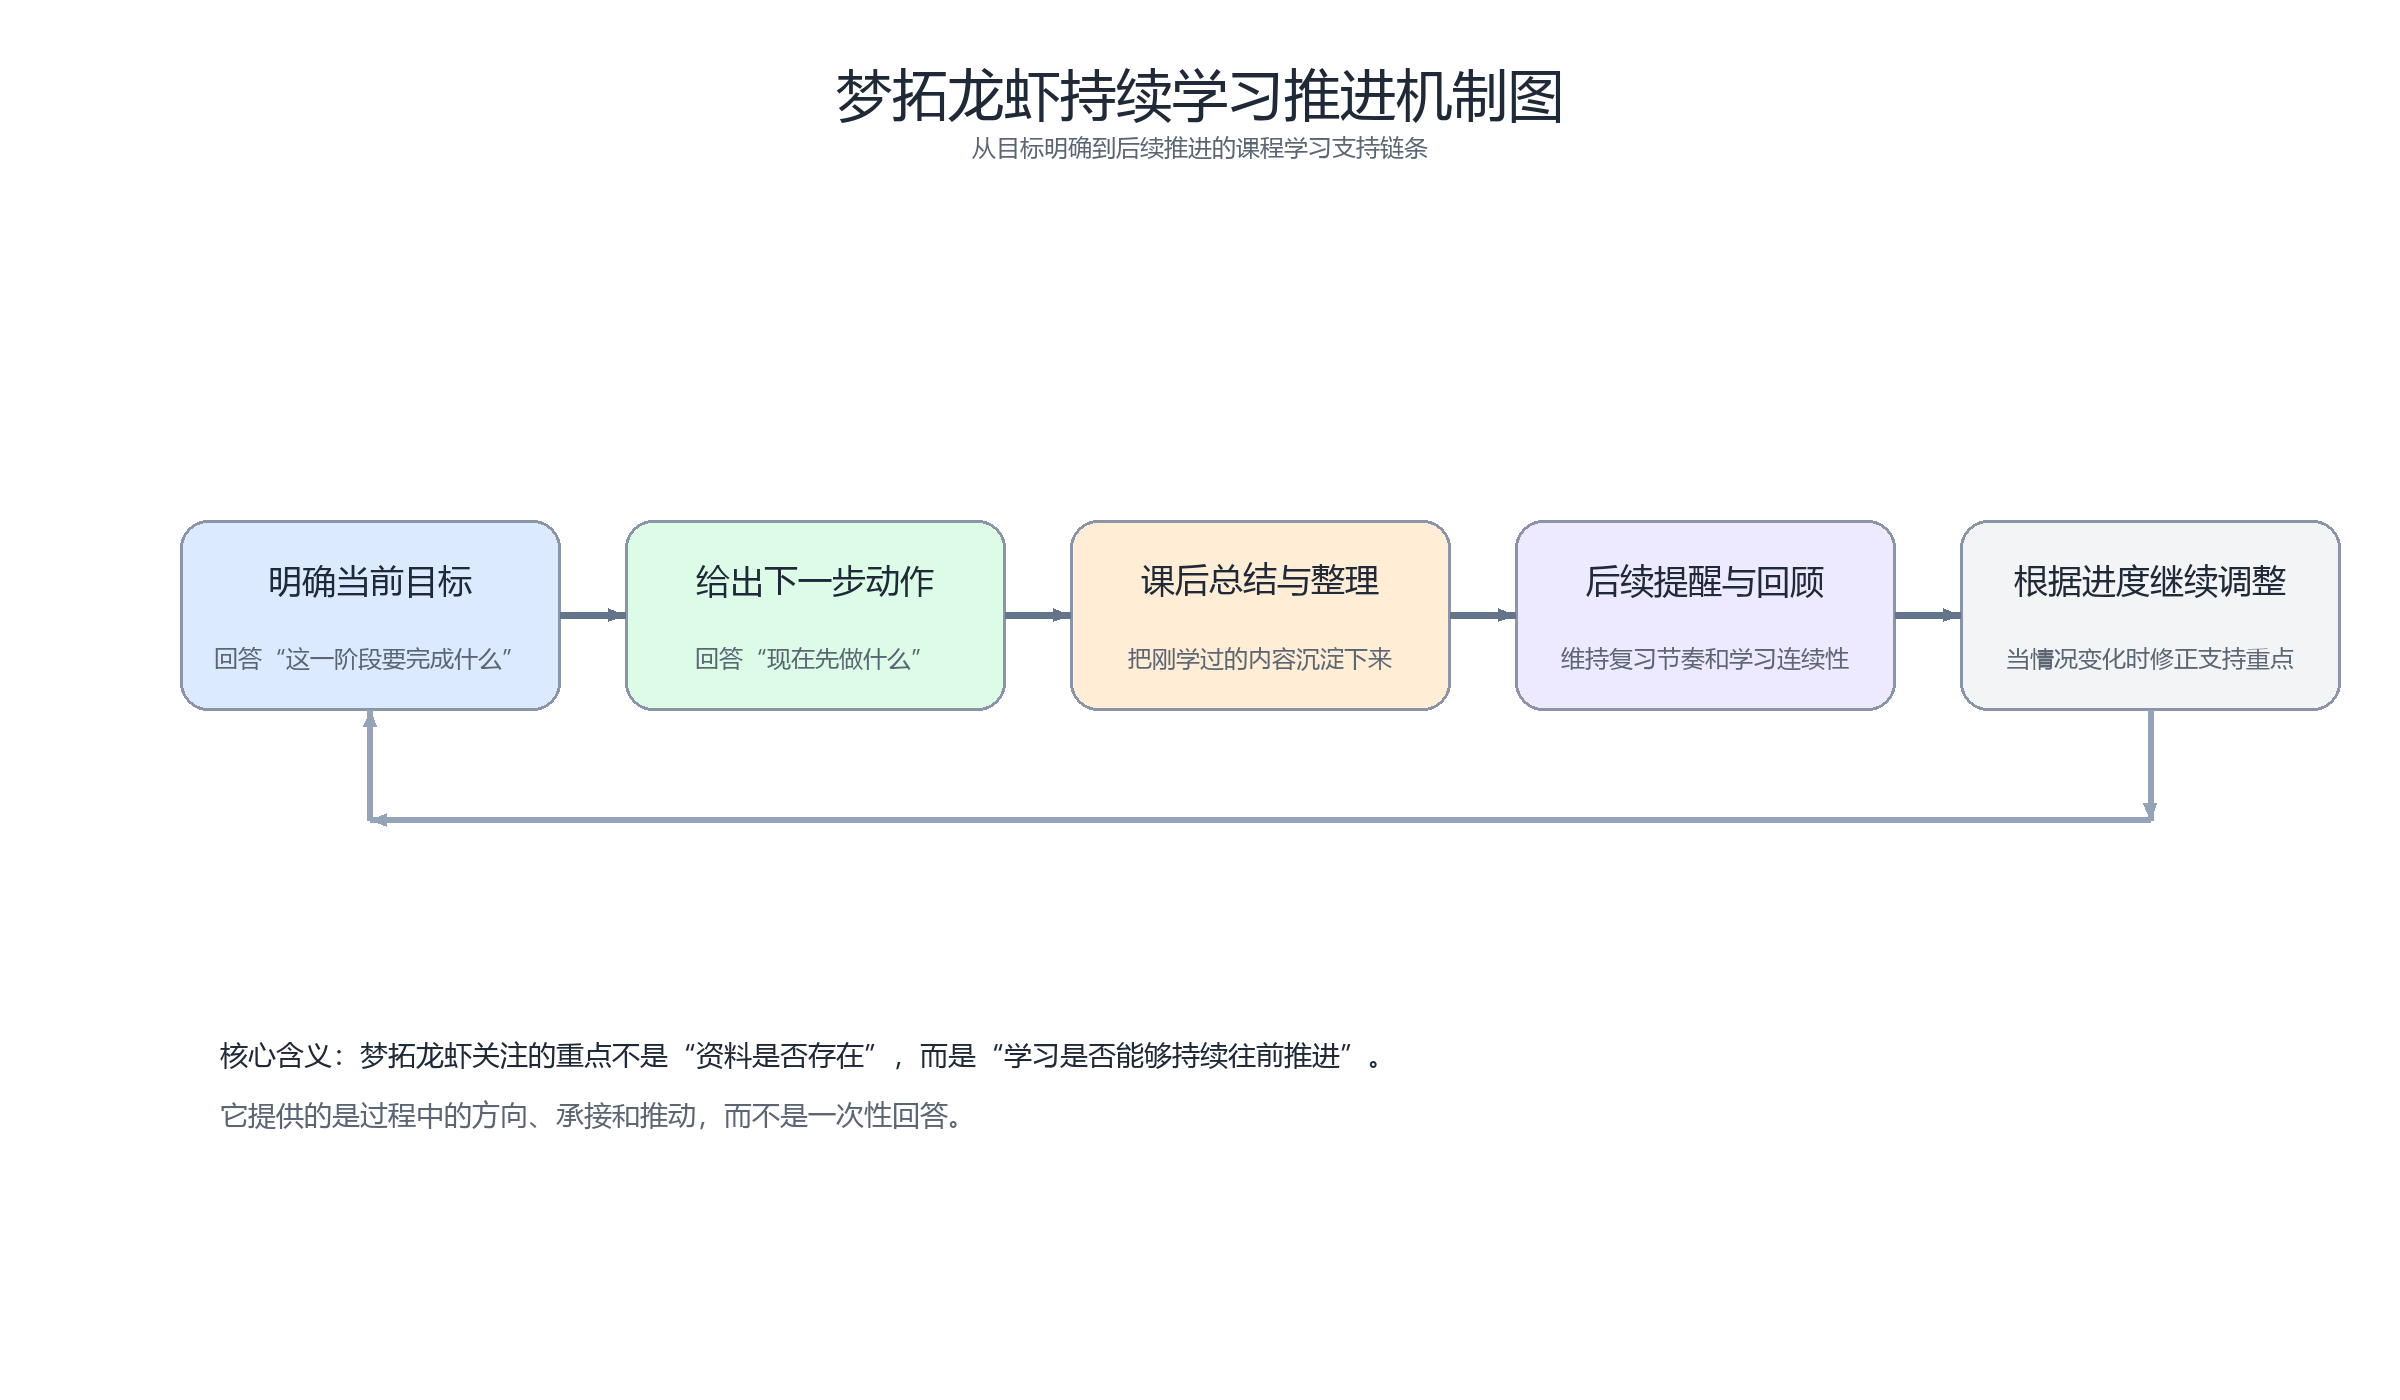
\includegraphics[width=0.92\textwidth]{figure1-learning-progress.png}
\caption{梦拓龙虾持续学习推进机制示意图}
\label{fig:progress}
\end{figure}

如图 \ref{fig:progress} 所示，梦拓龙虾并不把课程学习看成一串孤立问题，而是看成需要持续承接的推进链路。目标建立回答“当前最值得推进什么”，任务推进回答“此刻先做什么”，课后复盘负责把刚学完的内容沉淀下来，周期复习负责在适当时机重新唤起关键知识点，动态调整则在时间安排、任务完成情况或理解程度变化时重新修正后续支持重点。

\subsection{总体架构}
围绕上述目标，梦拓龙虾采用由用户交互、学习编排、课程资料和支持输出构成的总体架构。用户交互层接收课程目标、课程内提问、课后复盘需求和主动任务设置；学习编排层负责识别当前处于哪类学习阶段，并组织后续支持动作；课程资料层负责接入课表、作业、课件、回放和通知等校内资源；支持输出层负责形成学习计划、课后总结、复习提醒和阶段检查等结果。

\begin{figure}[H]
\centering
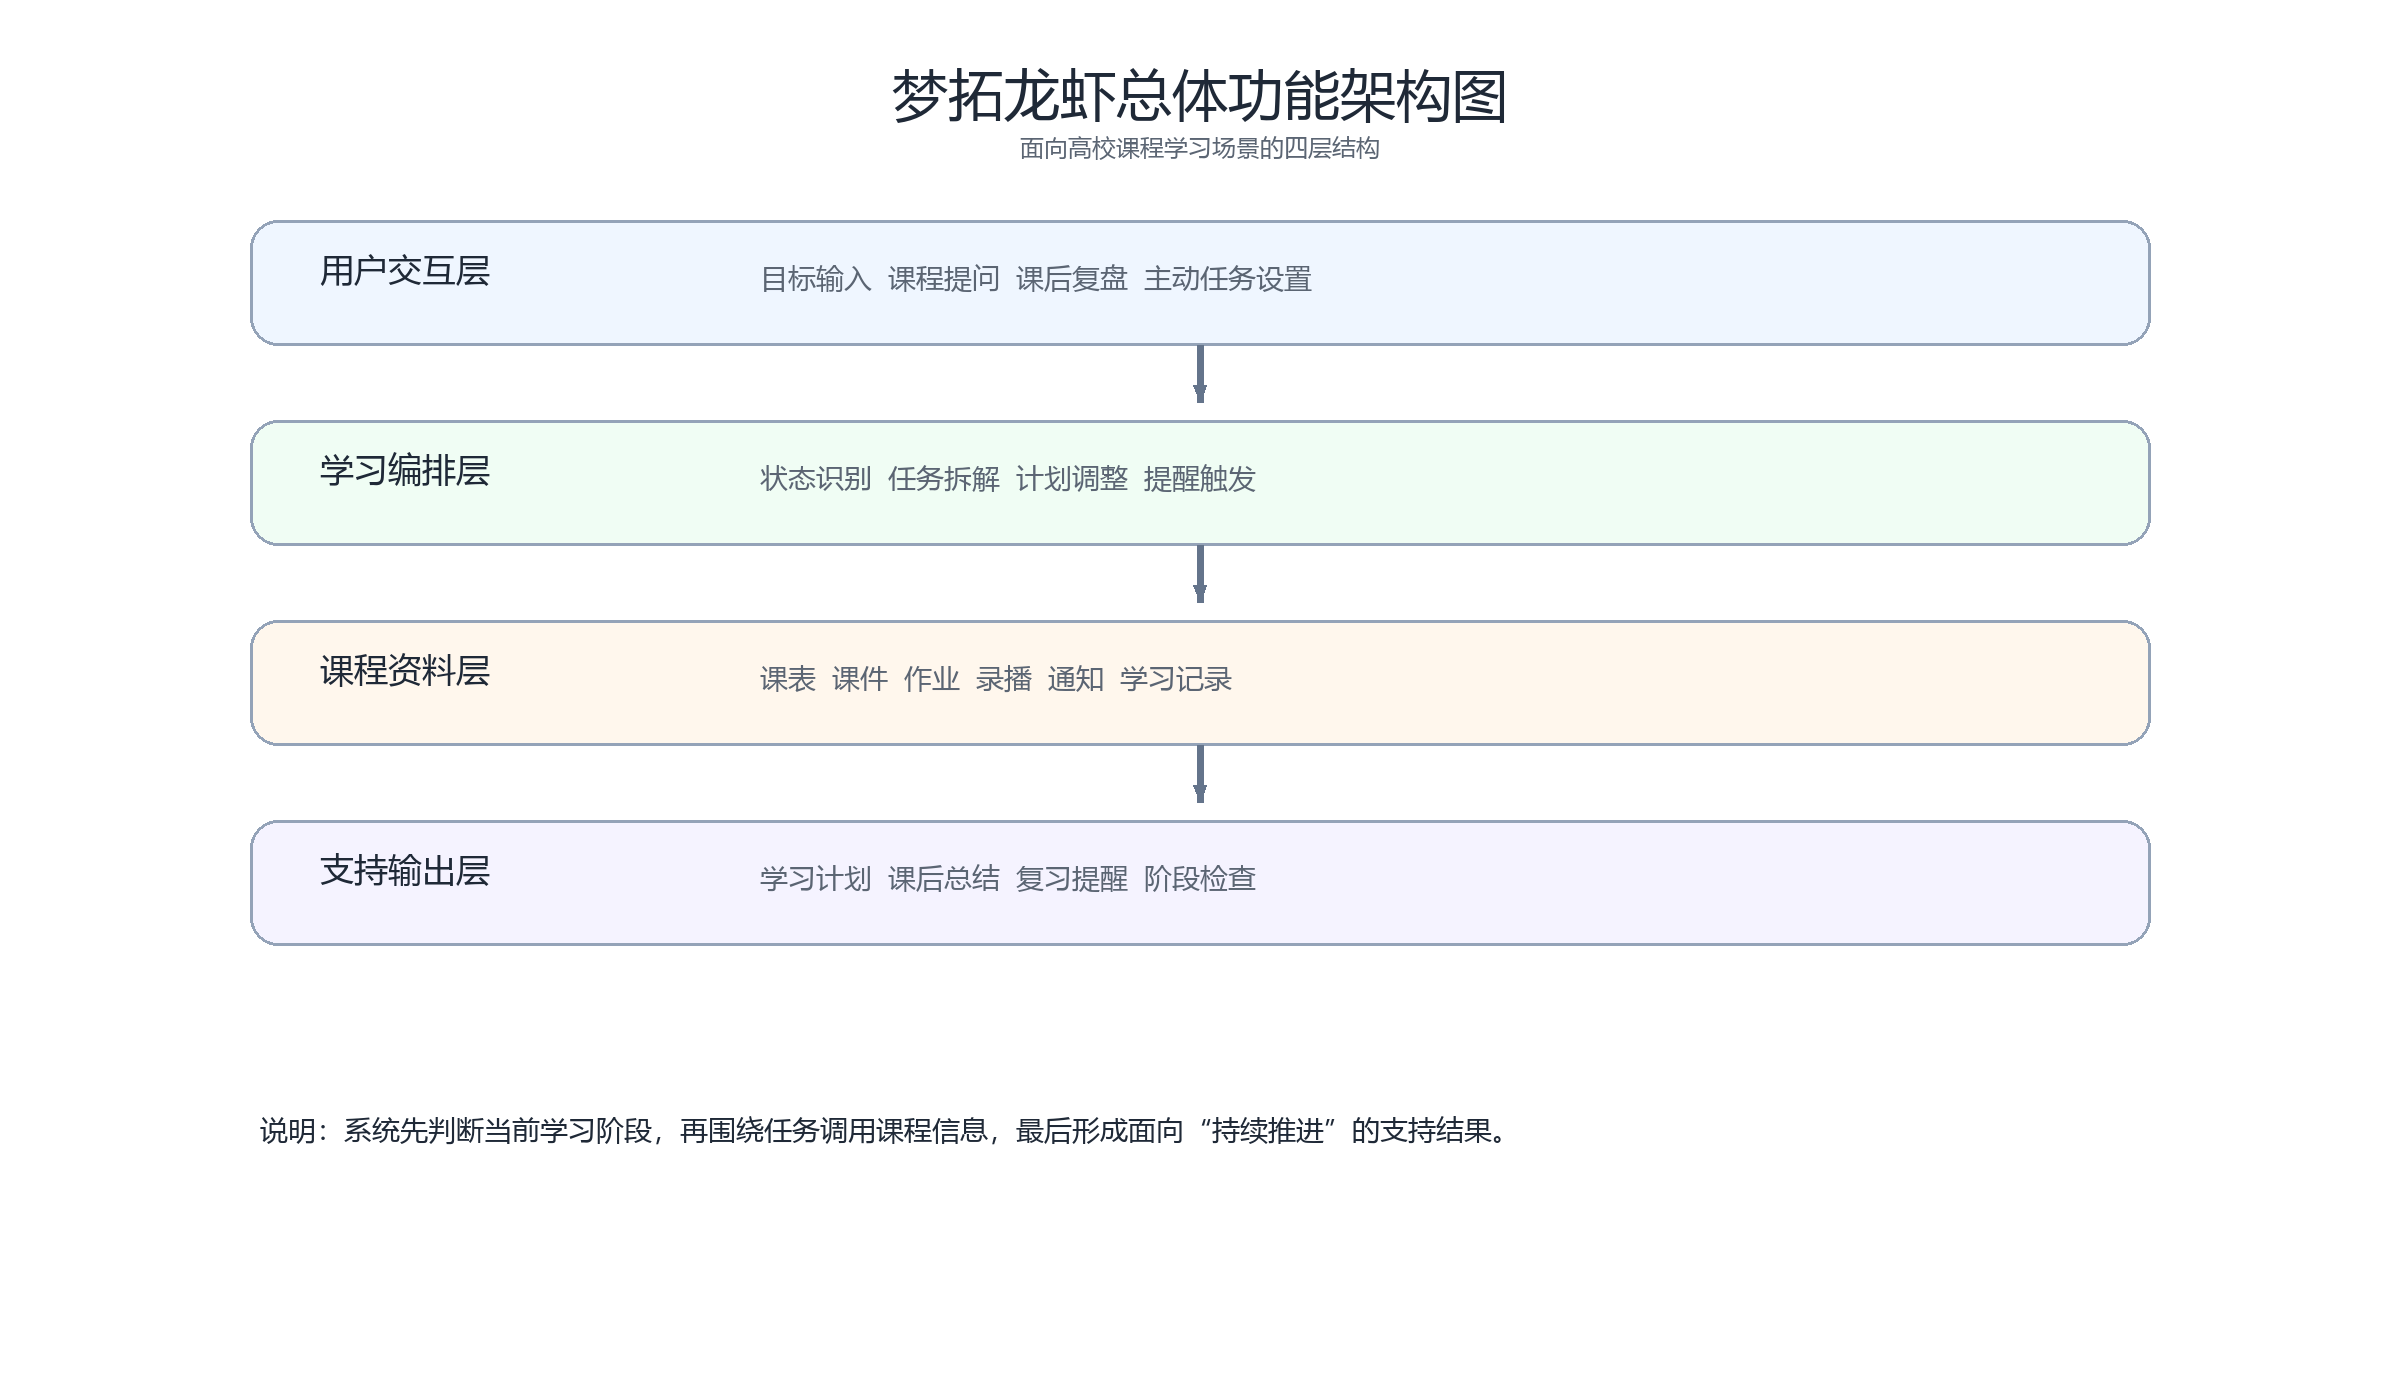
\includegraphics[width=0.92\textwidth]{figure2-architecture.png}
\caption{梦拓龙虾总体功能架构图}
\label{fig:architecture}
\end{figure}

图 \ref{fig:architecture} 反映的关键思想是：课程资源不是系统存在的目的，而是支撑系统完成课后监督与持续推进的依据；学习编排层不是单纯做信息路由，而是要根据当前课程状态决定“现在最值得做的支持动作”。

\subsection{核心对象设计}
为了让学习支持既能长期持续，又不至于把所有状态混在一起，梦拓龙虾围绕三个核心对象组织运行。

第一，学习者对象。该对象用于记录较稳定的学习偏好、时间习惯、常见薄弱点和近期风险信号。它不追求一次性建成复杂画像，而强调记录真正影响后续支持方式的长期信息。

第二，课程项目对象。课程项目是梦拓龙虾的核心业务单元，通常对应某门课在某一阶段的推进目标，例如“本学期《信号与系统》的日常学习支持”或“期中复习推进”。对象中保存课程绑定关系、当前目标、最近进展、待推进任务以及后续关注重点。

第三，cron 任务对象。cron 任务用于承接那些需要重复发生的主动支持行为，例如每节课后当晚推送复盘内容、每周检查某门课的作业进展、考试前一周启动强化复习等。相比一次性对话，cron 任务更能体现梦拓龙虾“持续推进”的作品特点。

\subsection{基本工作流程}
梦拓龙虾的典型运行链路如下：首先，用户创建课程项目或在已有课程项目中发起提问；其次，系统结合当前课程状态判断本次需求更偏向目标建立、即时支持、课后复盘还是复习推进；然后，系统从相关课程资源中提取最小必要上下文，避免把无关资料大量堆叠到当前任务中；接着，系统输出当前最有价值的支持内容，如下一步任务、课后总结、知识点提醒或小题检查；最后，系统根据用户反馈和任务结果更新课程项目状态，并等待下一次用户触发或 cron 触发。

其中，用户触发和 cron 触发共同构成了梦拓龙虾的工作入口。前者解决“学生主动寻求帮助”时的支持问题，后者解决“学生没有主动提问但仍需要被拉回学习过程”时的问题。这一双入口设计正是系统区别于普通问答助手的重要原因。

\section{关键机制设计与实现}
\subsection{面向持续推进的学习状态建模机制}
梦拓龙虾并不把学习状态建模理解为对每个知识点进行复杂打分，而是围绕“如何决定下一步支持动作”维护一组足够有效的状态信号。这些信号主要包括：课程当前阶段、最近一次推进任务是否完成、近期是否出现理解困难、课后复盘是否中断、复习是否被拖延，以及学生更适合接受何种形式的支持。

这种设计的出发点很直接。对于课程持续推进而言，真正关键的问题不是“系统是否精确知道学生掌握度的绝对值”，而是“系统是否能及时发现学生正在掉队，并及时给出下一步支持”。因此，梦拓龙虾优先维护与推进决策直接相关的状态，而不是追求庞大却难以落地的全量认知模型。相关思路与学习者知识追踪研究关注长期学习状态的思想具有一致性\cite{corbett1994}，但在原型阶段更强调轻量、可执行和可持续维护。

\subsection{课程资源接入与最小上下文构建机制}
课程资源接入是梦拓龙虾能够真正参与课程学习过程的前提。在北航场景下，原型主要围绕校内教务课表与课程资源平台工作，其中课表信息提供课程与上课时间真相，课程平台进一步提供作业、通知、回放和课件等学习资源。系统并不把“资源接得越多越好”作为目标，而是强调课程资源必须为当前推进任务服务。

因此，在具体调用时，梦拓龙虾采用最小必要上下文构建策略。若用户询问的是本周任务，系统优先调用课程项目中的任务状态与作业信息；若需求发生在课后复盘场景，系统优先调用最近一次课堂相关的回放、课件和通知内容；若进入复习场景，系统则优先提取前期已经标记为关键或易错的知识点。通过这种方式，系统避免把大量无关资源推给模型或学生，从而提高支持内容的针对性和可执行性。

\subsection{课后监督与复盘机制}
课后监督是梦拓龙虾当前最具代表性的设计重点。其核心思想不是“自动生成一段总结文字”，而是在课程刚结束、遗忘尚未加深时，迅速把课堂内容重新组织为可巩固、可检查的课后支持内容。这一机制尤其适合通过定时任务来实现，因为学生最容易在离开课堂后被其他事务打断，若没有外部推动，复盘行为很容易被拖延。

在典型场景中，用户可以为某门课设置 cron 任务：每节课结束后，于当天晚上固定时间触发一次课后监督。系统在触发时首先定位最近一次课堂或课程回放，再结合课程项目已有状态，生成适合当晚完成的支持内容，例如三到五个核心知识点、一到两道用于自测的小题，或一段明确指出“今天最容易忽略的概念”的提醒。与泛化提醒相比，这种机制的关键优势在于它直接绑定具体课程、具体课次和具体内容，因此能够同时兼顾复习和评估两种作用。

\subsection{周期复习与动态调整机制}
只进行一次课后复盘仍然不足以支持长期保持。根据分散练习和提取练习研究，学习效果需要通过后续多次唤起和检查来稳定保持\cite{cepeda2006,dunlosky2013,karpicke2011}。基于这一认识，梦拓龙虾在课后监督之外进一步设计了周期复习机制。系统会根据课程项目中的近期重点、历史复盘结果和任务完成情况，在之后的合适时机再次推送复习要点、小题或提醒内容。

与此同时，梦拓龙虾还强调动态调整。现实学习中，学生的课程节奏经常变化：某周作业增多、某次课没听懂、某门课被迫临时降优先级，都会使原有路径失效。因此，系统需要根据用户反馈和近期执行情况及时调整任务粒度、提醒频率和关注重点，而不是机械重复原有计划。梦拓龙虾现阶段已经具备围绕课程项目做轻量调整的能力，这使其更接近真实学习场景中的陪伴式支持，而非静态计划单。

\subsection{个性化 cron 自动化机制}
为了让主动支持长期稳定发生，梦拓龙虾引入了个性化 cron 自动化机制。用户可以围绕课程或课程项目定义重复性任务，例如“每节课后当晚推送巩固内容”“每周日晚检查本周作业与遗漏知识点”“考试前一周每天提醒高频易错点”等。cron 任务的核心价值不在于“定时”本身，而在于把课程支持从偶发交互转化为可持续执行的外部机制。

需要理性说明的是，梦拓龙虾当前原型的成熟部分主要体现在 cron 任务的语义表达、课程绑定和支持内容生成逻辑上；而完整的产品级调度链路、通知通道和更复杂的触发条件仍有进一步完善空间。也就是说，本文强调的是作品已经建立了“主动执行课程支持”的核心框架，而不是声称所有自动化细节都已完全产品化。

\subsection{原型实现}
梦拓龙虾原型基于 OpenClaw 运行时实现，其中通用会话管理、基础调度钩子等能力由运行时提供，而围绕课程资源接入、课程项目组织、课后监督逻辑和 cron 任务语义的设计与实现由梦拓龙虾自身完成。这样的实现方式符合系统定位：尽量复用成熟通用能力，把主要精力集中在高校课程学习场景独有的问题上。

从原型能力看，系统已经能够围绕课程建立项目，接入校内课程资源，围绕特定课程课次构造支持上下文，并基于定时任务触发课后监督和复习支持。相比把精力投入到通用聊天框架的重复实现，这种做法更能体现作品在创意赛道中的实际价值。

\section{场景验证与分析}
\subsection{验证目标}
本文的验证重点并不是比较模型在某道题上的单次回答优劣，而是观察梦拓龙虾是否能够在真实课程场景中形成持续推进作用。换言之，本文更关注以下问题：系统能否把学习目标稳定绑定到具体课程；能否在课后自动生成有针对性的复盘与巩固内容；能否在后续时间再次把学生拉回复习任务；能否根据任务完成情况调整后续支持。

\subsection{典型场景验证}
围绕上述目标，本文选取四类典型场景进行验证。

\begin{enumerate}[leftmargin=2em,itemsep=2pt,topsep=4pt]
\item 新课程项目创建与目标建立。系统围绕一门具体课程创建课程项目，记录当前阶段目标、最近任务与后续推进重点，避免学习支持始终停留在零散提问层面。
\item 课后定时监督推送。系统为课程绑定课后 cron 任务，在课程结束后的当日晚间，结合最近一次课程回放相关内容，推送核心知识点、小题或提醒，用于帮助学生完成当天复盘与初步评估。
\item 周期复习与状态更新。系统依据前期复盘与推进情况，在后续时间继续推送复习内容，并根据用户反馈更新当前重点与提醒频率。
\item 用户自定义主动任务。用户可以根据个人习惯设置不同频率和目标的任务，如周检、考前强化或遗漏知识点追踪，以体现系统的可扩展性与个性化特征。
\end{enumerate}

\begin{figure}[H]
\centering
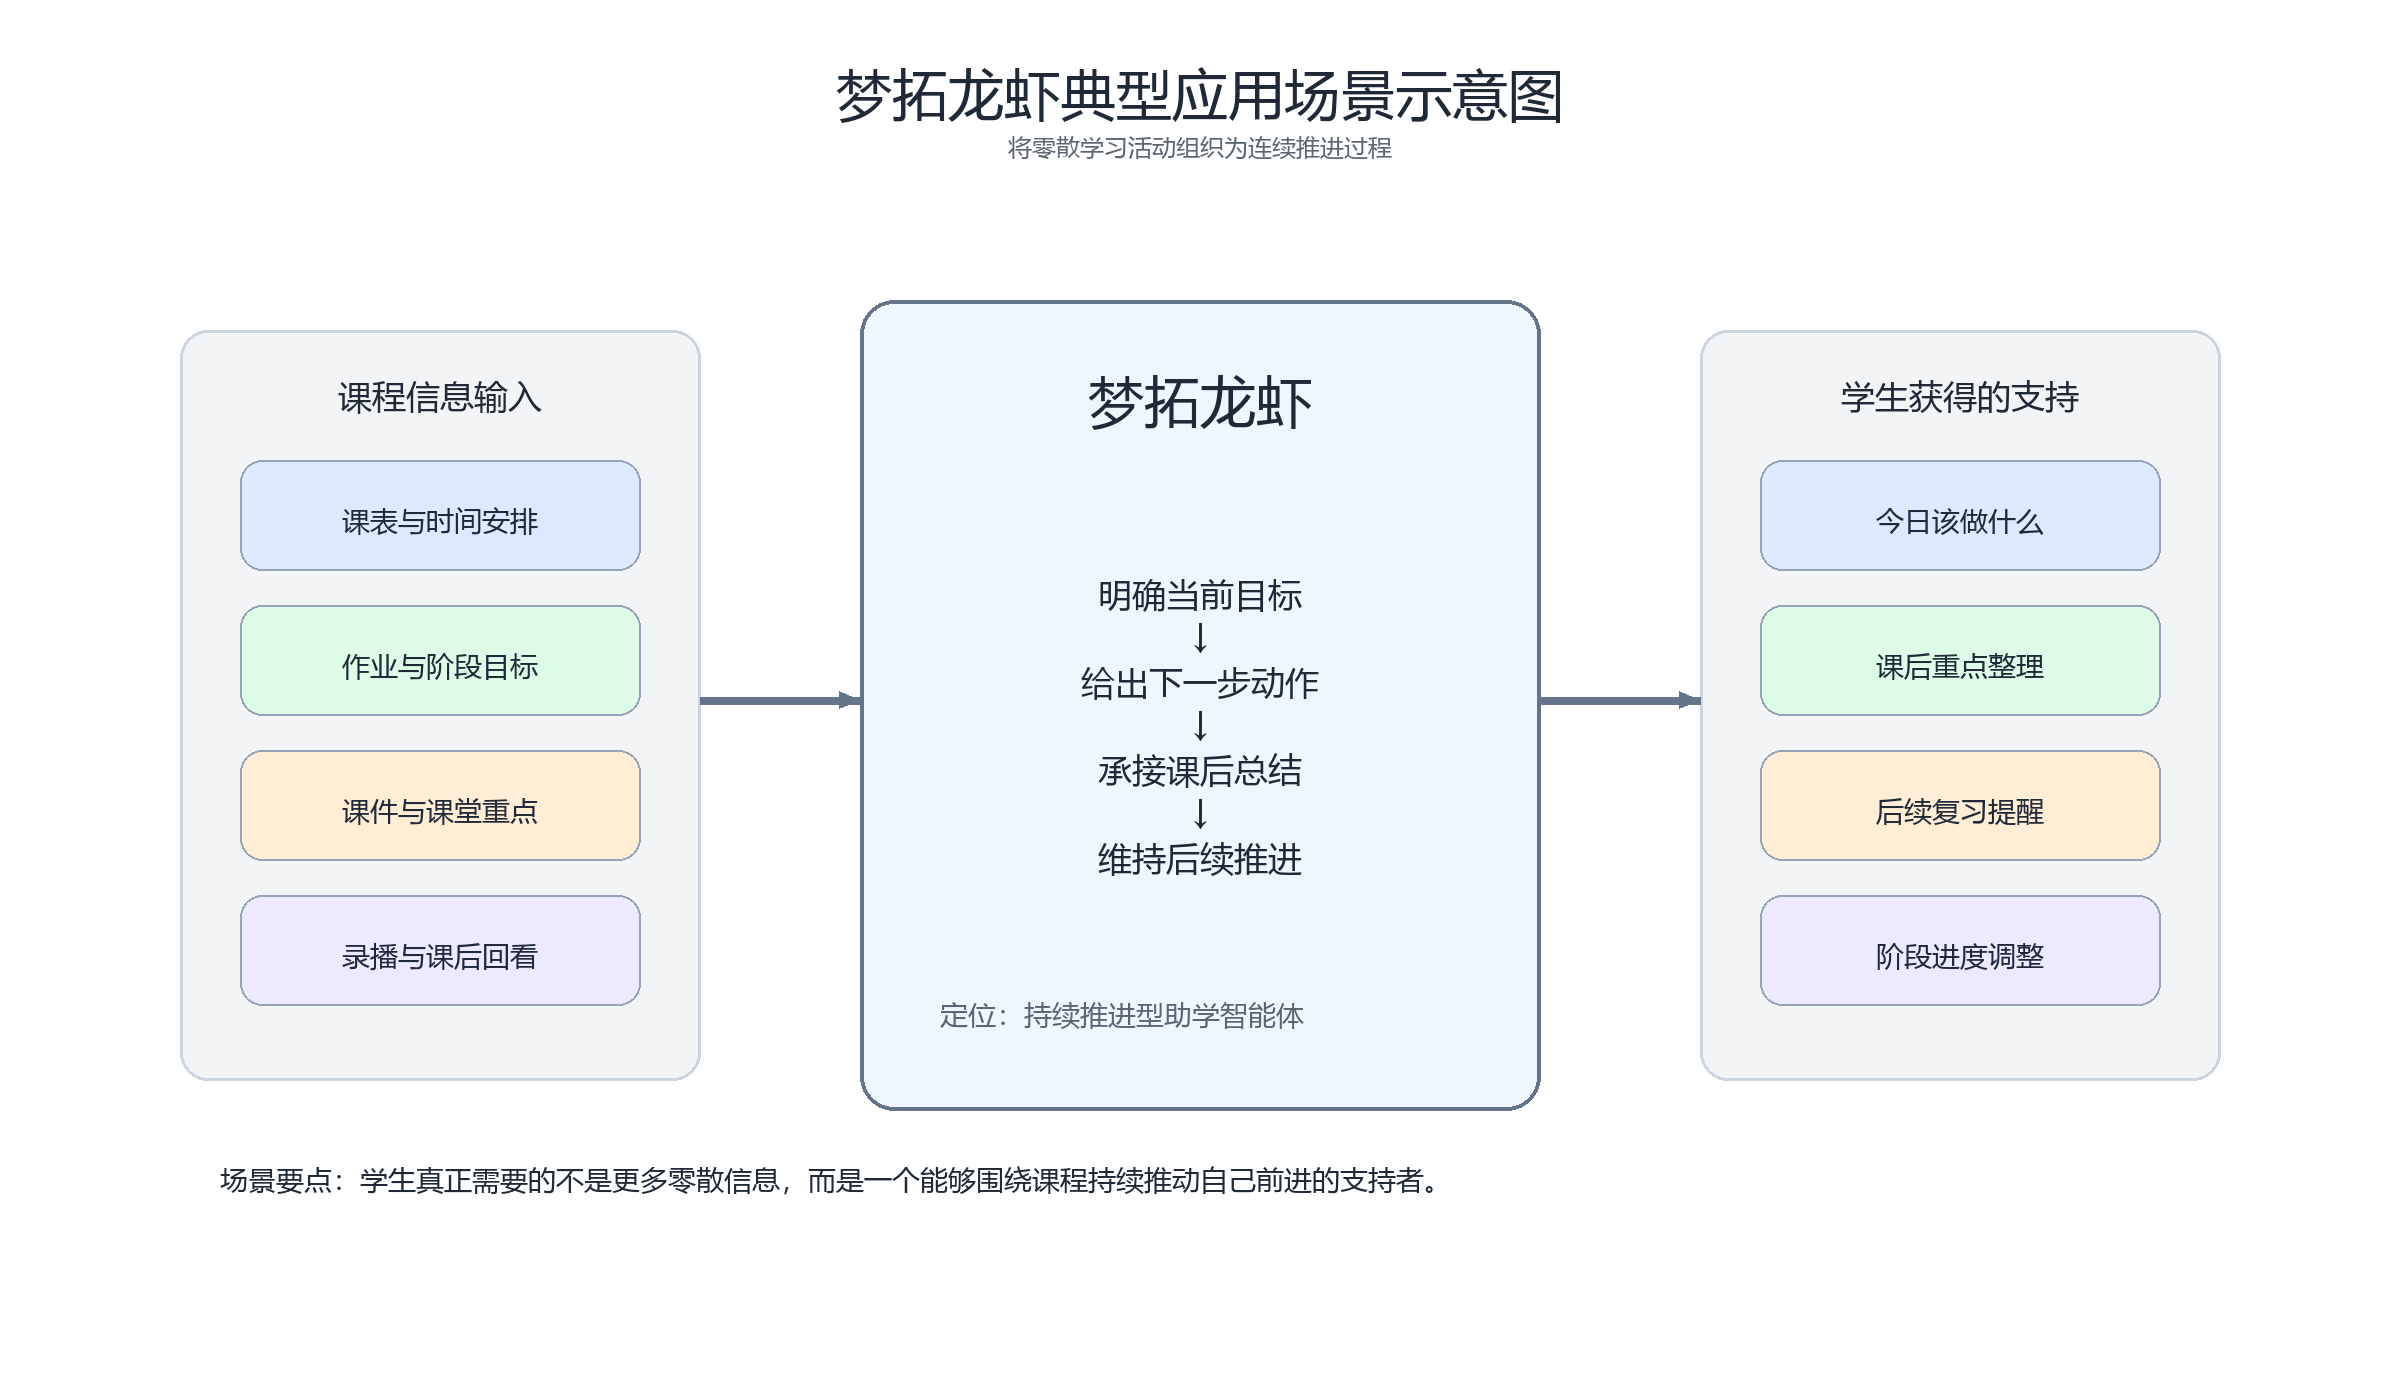
\includegraphics[width=0.92\textwidth]{figure3-scenario.png}
\caption{梦拓龙虾典型应用场景示意图}
\label{fig:scenario}
\end{figure}

图 \ref{fig:scenario} 所示的正是梦拓龙虾最具代表性的使用方式：系统从校内课程平台获取与当前课程相关的信息，再围绕课后复盘、当日巩固和后续复习形成主动支持输出。相比传统平台“等学生自己回来找资料”，这种方式更强调系统对学习节奏的主动承接。

\subsection{结果分析}
从场景验证结果看，梦拓龙虾目前已经能够支撑课程学习中的几项关键能力。其一，系统能够把学习支持稳固地绑定到具体课程和具体阶段目标上，使后续互动不再是无上下文的零散提问。其二，系统能够在课后场景中基于课程资源生成针对性较强的复盘与巩固内容，从而承担一定的监督作用。其三，系统能够通过 cron 任务把复习和检查继续延伸到课后之后的时间段，使学习支持不局限于课堂结束当下。其四，系统能够根据任务推进情况对后续支持做出轻量调整，提高实际可用性。

这些能力的价值在于，它们把课程学习中的“知道很多”转化为“持续推进一点点”。对于高校课程学习而言，后者往往比单次问答更接近真实痛点，也更有可能在长期上产生效果。

\subsection{局限与难点}
尽管如此，梦拓龙虾当前仍存在若干局限。首先，系统对课程内容的理解仍然较多依赖已有资源质量，若课程回放、课件或通知不完整，则课后监督内容的质量会受到影响。其次，自动化机制的业务语义已经较为清晰，但完整的产品级触发、通知和多端交互链路仍需继续完善。再次，当前对学习效果的评估更多体现为任务完成、复习触发和用户反馈层面的过程性指标，尚未形成严格的长期学习成效测量体系。最后，不同课程之间的负荷协调仍较为初步，未来还需要进一步考虑多课程并行时的提醒节奏与优先级冲突问题。

\section{应用前景}
梦拓龙虾在高校课程学习、阶段性复习和自主学习督导等场景中具有较好的应用前景。随着校内平台逐步沉淀更多课程过程数据，助学智能体有机会从“答疑工具”进一步演化为“过程型学习支持者”。对于日常课程学习，它可以承担课后复盘和持续提醒的角色；对于期中、期末等阶段性任务，它可以围绕重点知识点和易错内容组织更高频的支持；对于自主学习场景，它还可以作为长期监督工具帮助学生维持节奏。

更重要的是，这一路径体现了一种值得继续发展的助学方向：真正有价值的助学智能体，不必追求成为全能型 AI，而应扎根于具体场景中的关键断点。对于高校课程学习而言，这个关键断点正是课后监督与持续推进。只要这一点能够被稳定建立起来，助学系统就有可能从“会回答问题”进一步走向“能陪学生把课学下去”。

\section*{结论}
本文围绕高校课程学习中“缺少持续推进机制”这一核心问题，设计并实现了助学智能体“梦拓龙虾”。系统依托校内课程资源平台，以课程项目和 cron 任务为主要组织方式，将目标建立、任务推进、课后复盘、周期复习和动态调整串联为持续运行的学习支持过程。特别是在课后监督场景中，梦拓龙虾能够结合课程回放相关内容，于课程结束后的当日晚间向学生推送核心知识点、小题或提醒信息，以帮助完成复习与评估。场景验证表明，该系统的核心价值不在于回答单个问题，而在于通过持续监督与主动推进，让课程学习过程保持连续、可承接、可调整。未来，随着课程资源理解深度、自动化链路和效果评估机制的进一步完善，梦拓龙虾有望在高校个性化助学中发挥更大作用。

\clearpage
\bibliography{references}

\end{document}
